\documentclass{scrartcl}
\usepackage{geometry}
\usepackage{csquotes}
\usepackage{hyperref}
\usepackage{graphicx}
\usepackage{float}
\usepackage{subcaption}
\graphicspath{ {images/} }

\geometry{legalpaper, portrait, margin=1in}
 
\title{Harvard University, John A. Paulson School of Engineering and Applied Sciences \newline}
\subtitle{CS236r Final Project\\ Computational Results For Peer-Prediction and Crowdsourced Judgement Elicitation}
\author{Virgile Audi (vaudi@g.harvard.edu)\\
		Charles Liu (cliu02@g.harvard.edu)}

\begin{document}
 
\maketitle
\section*{Introduction}

A common theme throughout the course is to question the practicality of mechanisms discussed in class. For our presentation of \emph{Crowdsourced Judgement Elicitation with Endogenous Proficiency} and \emph{Eliciting Informative Feedback: The Peer-Prediction Method}, we found the mechanisms relied on strong assumptions that were generally unrealistic. Also, as seen in the second homework with specifying learning rates, in many situations a model can be very sensitive to its parameterization. Difficulties in finding proper parameters can also be viewed as a potential flaw of the mechanism, making it unsuitable for use in a practical setting. For our final project we wanted to take a deeper look at the two mechanisms, relax their assumptions, and see if the mechanism can be modified to achieve similar results.

\section{Crowdsourced Elicitation}

The \emph{Crowdsourced Judgement Elicitation with Endogenous Proficiency} paper dealt with a model that incorporated three variables: effort, proficiency, and truthfulness. A user would be given a set of tasks, with each task having a binary type H or T. A user first has the binary option of giving full or no effort. On no effort, the user reports H/T based on a random coin flip. On full effort, the user then has a probability corresponding to his proficiency of correctly interpreting the event. Finally, he can report his signal either truthfully or untruthfully. 

An example use case for this kind of mechanism would be in grading assignments for massive open online courses (MOOCs). If there was a need for graders, e.g. assignments with non-numerical or multiple choice answers, it would be infeasible for a staff to consistently grade answers from thousands of students. Instead, having peer grading would be a natural solution conditional on the fact that students will take the time to grade the assignments and truthfully report the scores.

\subsection{Computational Results of Paper}

We first confirmed the results from the paper computationally, given all of their assumptions. The main benefit to this mechanism was that the maximum reward was achieved in the equilibrium where everyone gave full effort and reported truthfully, whereas giving no effort resulted in an expected reward of 0. Giving full effort and reporting untruthfully is also an equilibrium, however this can be remedied by having some ``known'' truthful users put into the mechanism. One of the stronger results from the paper was Lemma 8:
 
\begin{displayquote}
Suppose the probability of agent i using strategy (1, X) is $\delta$ and strategy $(0, r_i)$ is $1-\delta$ for each task $j \in J(i)$. Suppose i'’s potential reference raters $r_j (i)$ use strategies (1, X) and $(0, r_{r_j} (i))$ with probabilities $\epsilon_{r_j}(i)$ and $1-\epsilon_{r_j}(i)$ respectively, for each task $j \in J(i)$. If $\epsilon_{r_j}(i) > 0$ for any reference rater with proficiency $p_{r_j} (i) > \frac{1}{2}$, then agent i has a (strict) profitable deviation to $\delta'=1$, i.e., to always using strategy (1, X), for all values of $r_i \in [0,1]$
\end{displayquote}

\begin{figure}[H]
	\caption{Computational results of different equilibriums vs. other strategies}
	\centering
	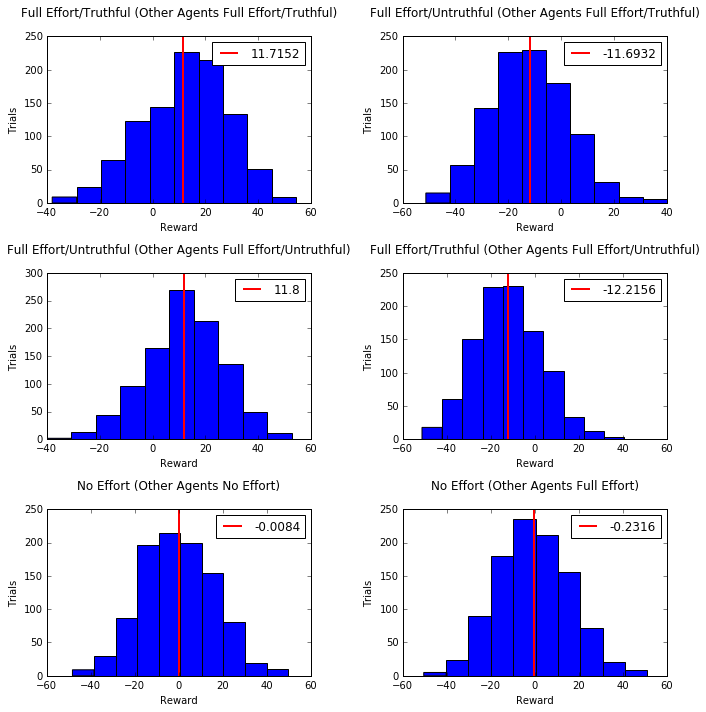
\includegraphics[width=1.0\textwidth]{cs_equilibriums}
\end{figure}
\begin{figure}[H]
	\caption{Computational results of Lemma 8}
	\centering
	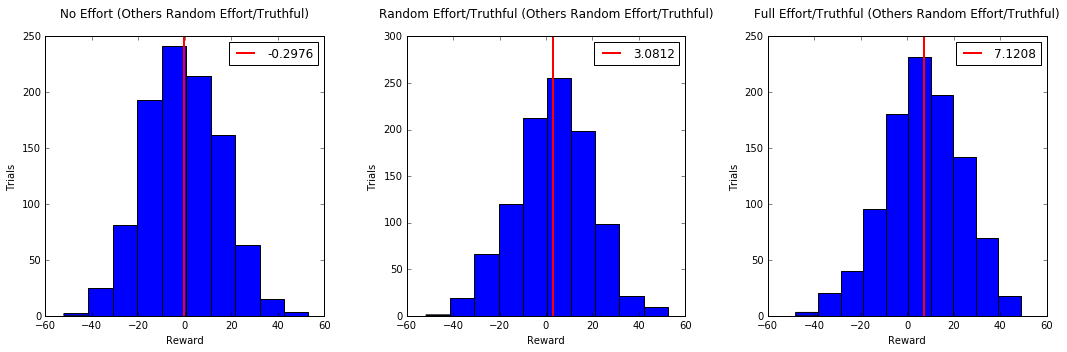
\includegraphics[width=1.0\textwidth]{cs_lemma8}
\end{figure}

Figure 1 is a summary of the main results and Figure 2 of Lemma 8. In each scenario, there were 100 tasks and 20 agents each performing 10 tasks. Simulations were run 1000 times, rewards were scaled by 10, and no costs were factored into the model. 

\section{Peer Prediction}

We recall the main assumptions made in the paper:

\begin{enumerate}
\item Conditional on the product’s type, raters’ signal sare independent and identically distributed, i.e. raters have common prior
\item Raters have common knowledge of the probability of reporting a signal given a type of a product.
\end{enumerate}

The objective of this project being to relax some of these assumptions, we implemented an agent class in python that would allow for different prior distribibutions as well as personal signal probability given the particular type of a product. We also implemented the various score functions mentioned in the paper, i.e. Quadratic, Spherical and Log scoring rules.

We then wanted to verify the main proposition of the paper:

\begin{displayquote}
For any mapping r that assigns to each rater i a reference rater r i  ̸= i, and for any proper scoring rule R, truthful reporting is a strict Nash equilibrium of the simultaneous reporting game with transfers  i∗ .
\end{displayquote}

To do so, we simulated 1000 experiments where 2 agents who satisfy the assumptions presented above, reports 1000 signals over two types. We fix agent 2 to always be truthful and let agent 1 be truthful, deceitful or even adopt a randomised strategy (0.5, 0.5). As we can see on figure 4, it seems to always be better to report truthfully, even if it is only slightly more advantageous than to report using a randomised strategy. This last statement could also be invalidated with further testing and different randomised strategies.\\

We also noted an interesting results when trying to relax the second assumption stated above. For Proposition 1 to hold, we in fact need not only that  raters have common knowledge of the probability of reporting a signal given a type of a product, but also that these distributions are to be the same. To validate this new assumption, we simulated the same experiments as before, but with agents having different distributions of perception, which is in fact close to the proficiency consideration of the crowd-sourcing paper. In one case, we used an agent that was rather undecided when receiving a signal, having a 50\% chance of correctly reading the signal. In the other, we designed an agent that was very bad at identifying the type for which the second agent is actually quite good at, and keeping the second type distribution the same. Figure 6 shows that to always lie is a better strategy for agent 1, if he knows that he tends to read signals worse than his refering agent !\\ 

Next steps of this part of the project woudl be to focus on this issue as well as relaxing the first assumption of common priors over types.
\section{Results}
\subsection{Peer Prediction}
\begin{figure}[H]
\caption{Computational verification of Property 1}
\begin{subfigure}{0.4\textwidth}
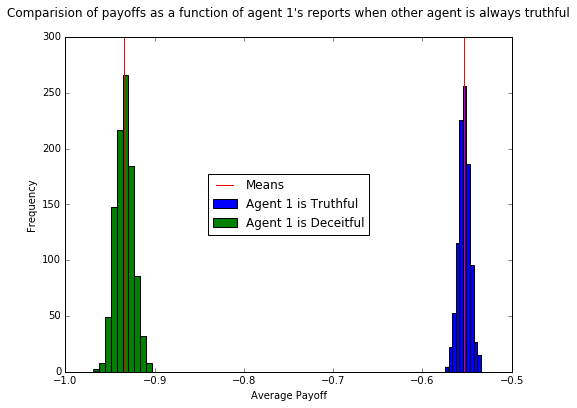
\includegraphics[scale=0.4]{pp_1}
\end{subfigure}
\hspace{0.1\textwidth}
\begin{subfigure}{0.4\textwidth}
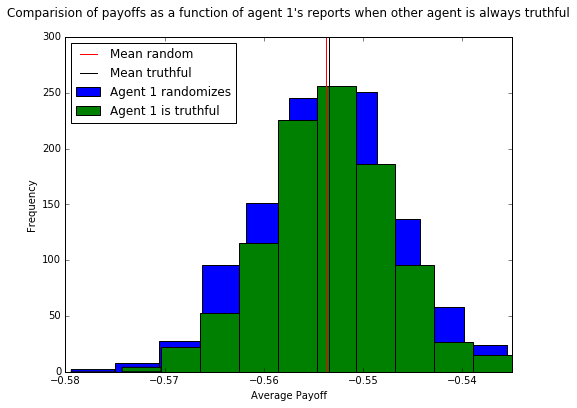
\includegraphics[scale=0.4]{rand}
\end{subfigure}
\end{figure}

\begin{figure}[H]
\caption{Relaxing Assumption 2}
\begin{subfigure}{0.4\textwidth}
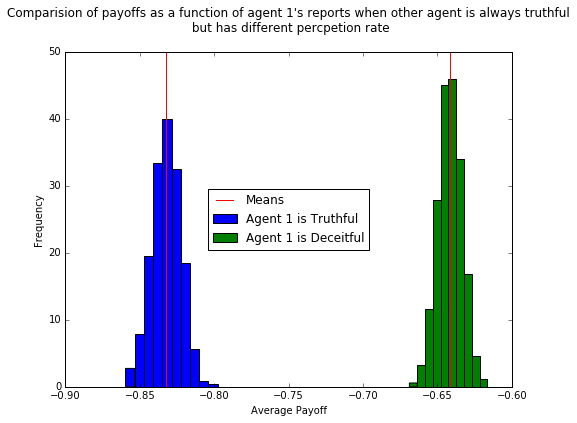
\includegraphics[scale=0.4]{pp_2}
\end{subfigure}
\hspace{0.1\textwidth}
\begin{subfigure}{0.4\textwidth}
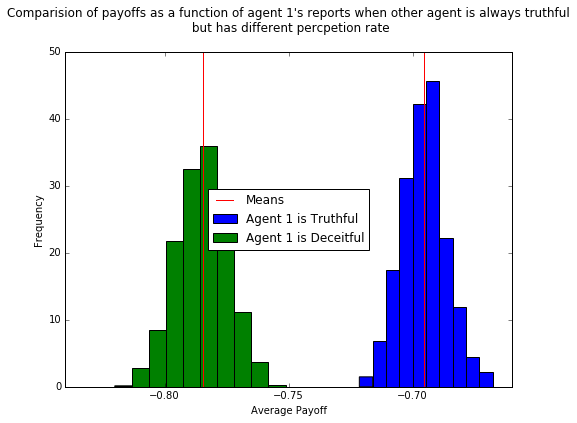
\includegraphics[scale=0.4]{pp_3}
\end{subfigure}
\end{figure}
\end{document}